%modificato in tesi.tex--> aggiunto \usepackage{verbatim}
\chapter{Filtri digitali}


\section{Denoising}

Uno degli ostacoli principali dell'analisi computerizzata dei suoni polmonari \`e la presenza di rumore nei segnali. 
In questo caso per rumore si intendono quei suoni provenienti da strumenti come ventilatore, aria condizionata, e altri rumori ambientali che possono contaminare i segnali sonori del polmone. 
La natura rumorosa dei suoni polmonari \`e un fattore di impedimento che vieta l'identificazione di funzioni utili per la diagnostica. 
Quindi il denoising di segnali sonori polmonari \`e d'obbligo per l'utilizzo efficace della diagnosi e in questo capitolo approfondiremo le varie tecniche per l'eliminazione dei rumori.

\section{Classificazione dei filtri digitali}

Un filtro digitale \`e una funzione in grado di modificare il contenuto armonico di un segnale elettrico complesso.
Queste modifiche si esprimono in termini di fasci di frequenze che vengono evidenziate o soppresse a seconda delle caratteristiche del tipo di filtro usato.
Una importante penalizzazione per i filtri digitali \`e che sono limitati nelle frequenze: un filtro digitale deve sempre e comunque rispettare il teorema di Nyquist, ovvero il teorema del campionamento, che impone al filtro un limite massimo sulle frequenze che pu\`o elaborare, altrimenti si ottengono segnali disturbati da aliasing.

Si distinguono due classi di filtri: lineari e non lineari.
\begin{description}
      \item[Filtri lineari]
	  La funzione d\`a in uscita un valore che \`e una combinazione lineare dei valori compresi nella finestra del segnale appena analizzato, cio\`e l'output del filtro pu\`o mettersi in relazione con i valori presi in ingresso. Si possono definire filtri lineari che puliscono il segnale dal rumore oppure che esaltano le discontinuit\`a.
      \item[Filtri non lineari]
	  Per questo tipo di filtro non \`e possibile definire un operatore lineare; solitamente sono operatori di rango, cio\`e operatori che agiscono sui valori presi in ingresso dopo averli ordinati quindi l'output dipende contemporaneamente da pi\`u ingressi.
 \end{description}
La differenza sostanziale tra i due tipi di filtri \`e che, mentre per i primi si pu\`o applicare la trasformata di Fourier con tutte le sue propriet\`a, nei secondi questa operazione non \`e possibile.

\subsection{Categorie di filtri}

I filtri si dividono in quattro principali categorie:

\subsubsection{Filtro passa alto}

Il filtro passa alto permette il passaggio di una banda di frequenze al di sopra di una determinata frequenza limite (\textit{frequenza di taglio}). Il taglio del filtro indica la zona della banda di frequenze che divide le due sezioni: frequenze passanti (alte), frequenze tagliate (basse).
\begin{figure}[h]
 \centering
 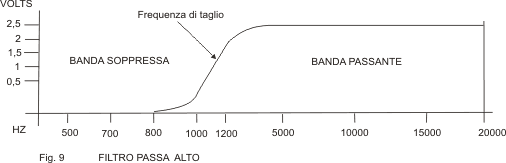
\includegraphics[width=0.6\textwidth]{./F_passa_alto.png}
  \caption{Esempio di un filtro passa alto \cite{SELET}}
 \end{figure}

\subsubsection{Filtro passa basso (low pass).}
Il filtro passa basso \`e esattamente l' opposto del filtro passa alto cio\`e permette il passaggio di una banda di frequenze al di sotto di una determinata frequenza limite. 

\begin{figure}[h]
 \centering
 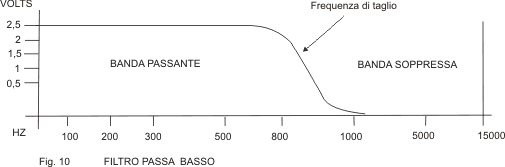
\includegraphics[width=0.6\textwidth]{./F_passa_basso.png}
 % F_passa_basso.png: 505x167 pixel, 72dpi, 17.81x5.89 cm, bb=0 0 505 167
  \caption{Esempio di un filtro passa basso \cite{SELET}}
\end{figure}



\subsubsection{Filtro passa banda (band pass).}
Il passa banda deriva dall'accoppiamento di un passa alto con un passa basso, quindi lascia passare solo una banda ristretta di frequenze che rientrano tra le frequenze di taglio dei due filtri accoppiati.
Comunque bisogna tener conto che al di sopra e al disotto di tali frequenze le altre componenti del segnale vengono eliminate, non in maniera netta, ma in modo graduale dipendente dalla "pendenza" della curva di selettivit\`a del filtro che varia a seconda del livello qualitativo del filtro stesso.

\begin{figure}[h]
 \centering
 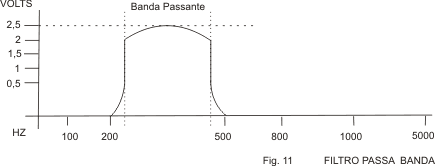
\includegraphics[width=0.6\textwidth]{./F_passa_banda.png}
 % F_passa_banda.png: 435x166 pixel, 72dpi, 15.34x5.86 cm, bb=0 0 435 166
 \caption{Esempio di un filtro passa banda \cite{SELET}}
 \end{figure}


\subsubsection{Filtro soppressore di banda (band reject).}
Il filtro a soppressione di banda \`e esattamente il contrario del filtro passa banda, in quanto pur essendo costituito dall'unione di un passa alto con un passa basso, respinge solo una ristretta banda di frequenze lasciando passare tutte le altre.

\begin{figure}[h]
 \centering
 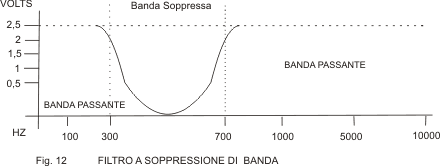
\includegraphics[width=0.6\textwidth]{./F_soppress_banda.png}
 % F_soppress_banda.png: 440x166 pixel, 72dpi, 15.52x5.86 cm, bb=0 0 440 166
 \caption{Esempio di un filtro soppressore di banda \cite{SELET}}
 \end{figure}

\section{Filtrare i suoni respiratori}
 
Entrando pi\`u nel dettaglio, durante l'analisi della letteratura attuale abbiamo riscontrato diversi tipi di filtri per l'eliminazione del rumore (denoising) e per eliminare il battito cardiaco.
L'eliminazione dei suoni emessi dal cuore \`e un problematica cruciale per il riconoscimento del respiro. 
Nello scenario previsto abbiamo un file audio del respiro preso grazie a uno stetoscopio elettronico; molti modelli di stetoscopi gi\`a concentono funzioni per filtrare il battito cardiaco, rilasciando quindi un suono a cui bisogna applicare solo un filtraggio per il denoising, per\`o nell'eventualit\`a in cui uno stetoscopio non sia fornito di queste funzioni bisogna trovare una tecnica di filtraggio ottimale che la maggior parte delle volte consiste nell'applicare piu di un filtro al suono che stiamo analizzando.
\newline
Si pu\`o subito notare attraverso l'analisi della letteratura approfondita nel capitolo 6, che il filtro usato maggiormente \`e quello passa banda, che permette di eliminare le frequenze che non rientrano nel range di frequenza dei suoni respiratori.
Per una migliore comprensione dell'analisi dei sistemi dei capitoli successi si andranno a illustrare alcune tecniche da loro usate.

\subsubsection{Downsampling }

Un filtro di downsampling o di sottocampionamento riduce la frequenza di campionamento di un segnale. Di solito lo scopo di questo filtro \`e di ridurre la complessit\`a computazionale dei successivi trattamenti del segnale. Il fattore di sottocampionamento \`e un numero intero o razionale maggiore di uno. Questo fattore moltiplica il tempo di campionamento o equivalentemente divide la frequenza di campionamento. Una implementazione di un filtro di sottocampionamento deve fare attenzione a non violare le condizioni del teorema sul campionamento di Shannon-Nyquist, altrimenti ci sar\`a la presenza di aliasing nel segnale di output. Questa tecnica viene usata sia da \cite{ASPODUOCSS} che da \cite{ASTFARA}.

\subsubsection{filtro mediano}

Il filtro mediano \`e un filtro non lineare ed \`e usato per la rimozione dei picchi di rumore dal segnale ed influenzano di solito solo una piccola percentuale dei campioni ma in modo notevole. L'idea principale di questo filtro \`e quella di rimpiazzare i campioni del segnale con la mediana dei campioni in una certo intervallo di campioni. Di solito questo intervallo si chiama finestra, la quale si muove su tutto il segnale campione per campione.

% \subsubsection{pacchetti wavelet}


\subsubsection{funzione finestra}
Nell'elaborazione numerica dei segnali una funzione finestra \`e una funzione che vale zero al di fuori di un certo intervallo. Quando un'altra funzione \`e moltiplicata per una funzione finestra, anche il prodotto assume valori nulli al di fuori dell'intervallo. Una definizione pi\`u generale di funzione finestra non richiede l'annullarsi al di fuori di un intervallo, ma che il prodotto per la funzione di finestra sia una funzione a quadrato sommabile, ovvero che la funzione finestra si annulli in maniera sufficientemente rapida. Le funzioni finestra sono importanti nel progetto dei filtri nell'analisi spettrale. 

% \paragraph{analisi spettrale}
% La trasformata di Fourier della fuzione $cos(\omega t)$ \`e zero tranne che alle frequenze $\pm \omega$. Quindi molte funzioni e forme d'onda non hanno una forma chiusa conveniente dalla trasformata. Alternativamente si potrebbe essere interessati nel contenuto spettrale durante un certo intervallo di tempo. In entrambi i casi, la trasformata di Fourier pu\`o essere applicata su uno o pi\`u intervalli finiti nella forma d'onda. In generale la trasformata \`e applicata al prodotto della forma d'onda e alla finestra. Ogni finestra influisce sulla stima spettrale calcolata con questo metodo. 
% 
% \paragraph{windowing}
% L'applicazione di una finestra ad una forma d'onda semplice come ad esempio $cos(\omega t)$ fa si che la sua trasformata di Fourier abbia valori diversi da zero in frequenze di verse da $\omega$. 
% If the waveform under analysis comprises two sinusoids of different frequencies, leakage can interfere with the ability to distinguish them spectrally. If their frequencies are dissimilar and one component is weaker, then leakage from the larger component can obscure the weaker one’s presence. But if the frequencies are similar, leakage can render them unresolvable even when the sinusoids are of equal strength.

% The rectangular window has excellent resolution characteristics for sinusoids of comparable strength, but it is a poor choice for sinusoids of disparate amplitudes. This characteristic is sometimes described as low-dynamic-range.
% 
% At the other extreme of dynamic range are the windows with the poorest resolution. These high-dynamic-range low-resolution windows are also poorest in terms of sensitivity; this is, if the input waveform contains random noise close to the frequency of a sinusoid, the response to noise, compared to the sinusoid, will be higher than with a higher-resolution window. In other words, the ability to find weak sinusoids amidst the noise is diminished by a high-dynamic-range window. High-dynamic-range windows are probably most often justified in wideband applications, where the spectrum being analyzed is expected to contain many different components of various amplitudes.
% 
% In between the extremes are moderate windows, such as Hamming and Hann. They are commonly used in narrowband applications, such as the spectrum of a telephone channel. In summary, spectral analysis involves a tradeoff between resolving comparable strength components with similar frequencies and resolving disparate strength components with dissimilar frequencies. That tradeoff occurs when the window function is chosen.Discrete-time signals
% 
% When the input waveform is time-sampled, instead of continuous, the analysis is usually done by applying a window function and then a discrete Fourier transform (DFT). But the DFT provides only a coarse sampling of the actual DTFT spectrum. Figure 1 shows a portion of the DTFT for a rectangularly windowed sinusoid. The actual frequency of the sinusoid is indicated as "0" on the horizontal axis. Everything else is leakage, exaggerated by the use of a logarithmic presentation. The unit of frequency is "DFT bins"; that is, the integer values on the frequency axis correspond to the frequencies sampled by the DFT. So the figure depicts a case where the actual frequency of the sinusoid happens to coincide with a DFT sample,[note 1] and the maximum value of the spectrum is accurately measured by that sample. When it misses the maximum value by some amount (up to 1/2 bin), the measurement error is referred to as scalloping loss (inspired by the shape of the peak). But the most interesting thing about this case is 
% that all the other samples coincide with nulls in the true spectrum. (The nulls are actually zero-crossings, which cannot be shown on a logarithmic scale such as this.) So in this case, the DFT creates the illusion of no leakage. Despite the unlikely conditions of this example, it is a common misconception that visible leakage is some sort of artifact of the DFT. But since any window function causes leakage, its apparent absence (in this contrived example) is actually the DFT artifact.
% 
% [edit]Noise bandwidth
% The concepts of resolution and dynamic range tend to be somewhat subjective, depending on what the user is actually trying to do. But they also tend to be highly correlated with the total leakage, which is quantifiable. It is usually expressed as an equivalent bandwidth, B. Think of it as redistributing the DTFT into a rectangular shape with height equal to the spectral maximum and width B.[note 2][4] The more leakage, the greater the bandwidth. It is sometimes called noise equivalent bandwidth or equivalent noise bandwidth, because it is proportional to the average power that will be registered by each DFT bin when the input signal contains a random noise component (or is just random noise). A graph of the power spectrum, averaged over time, typically reveals a flat noise floor, caused by this effect. The height of the noise floor is proportional to B. So two different window functions can produce different noise floors.
% 
% [edit]Processing gain
% In signal processing, operations are chosen to improve some aspect of quality of a signal by exploiting the differences between the signal and the corrupting influences. When the signal is a sinusoid corrupted by additive random noise, spectral analysis distributes the signal and noise components differently, often making it easier to detect the signal's presence or measure certain characteristics, such as amplitude and frequency. Effectively, the signal to noise ratio (SNR) is improved by distributing the noise uniformly, while concentrating most of the sinusoid's energy around one frequency. Processing gain is a term often used to describe an SNR improvement. The processing gain of spectral analysis depends on the window function, both its noise bandwidth (B) and its potential scalloping loss. These effects partially offset, because windows with the least scalloping naturally have the most leakage.



% Le finestre vengono usate spesso nel progetto dei filtri digitali, in particolare per convertire 
% Windows are sometimes used in the design of digital filters, in particular to convert an "ideal" impulse response of infinite duration, such as a sinc function, to a finite impulse response (FIR) filter design. That is called the window method.[5][6]


% \subsection{Esempi di finestre}

% \paragraph{terminologia}
% Usiamo $N$ per rappresentare l'ampiezza in numero di campioni di una finestra simmetrica $w(n)$. Se $N$ \`e un numero dispari, la finestra non-flat ha un unico punto singolare massimo. Se $N$ \`e pari, ha un doppio massimo. 
% La finestra cosidetta DFT-pari \`e asimmetrica e ha un solo massimo ma un numero pari di campioni(richiesti dall'algoritmo FFT). 
% Each figure label includes the corresponding noise equivalent bandwidth metric (B)[note 2], in units of DFT bins. As a guideline, windows are divided into two groups on the basis of B. One group comprises 1 ≤ B ≤ 1.8, and the other group comprises B ≥ 1.98. The Gauss, Kaiser, and Poisson windows are parametric families that span both groups, though only one or two examples of each are shown.
% Ci sono varie finestre ad esempio: finestra rettangolare \`e la pi\`u semplice, lascia invariati i campioni al suo interno e mette a zero gli altri. 
Siano $N$ l'ampiezza in numero di campioni di una finestra (tipicamente una potenza di 2) ed $n$ un numero intero, che assume valori da $0$ ad $N-1$. Ci sono varie funzioni finestre, ad esempio: 
  \begin{itemize}
    \item 
      la finestra rettangolare descritta dall'equazione 
      \[
	w(n)=1  
      \]
    \item
      la finestra di Hamming descritta dall'equazione
      \[
	w(n)=0.54-0.46 cos \left(\frac{2 \pi n}{N-1}\right)
      \]
      \`e stata progettata per minimizzare il livello del lobo laterale, mentre mantiene approssimativamente la stessa larghezza del lobo principale.
    \item
      la finestra di Hann o Hanning descritta dall'equazione:
      \[
	w(n)=0.5 cos \left(1-\frac{2 \pi n}{N-1}\right)
      \]
    \item
      la finestra di Blackmann descritta dall'equazione:
      \[
	w(n)=\frac{1-0.16}{2} - \frac{1}{2} cos \left(1-\frac{2 \pi n}{N-1}\right) + \frac{0.16}{2} cos \left(\frac{4 \pi n}{N-1}\right)
      \]
  \end{itemize}

% Other windows are designed to moderate these sudden changes because discontinuities have undesirable effects on the discrete-time Fourier transform (DTFT) and/or the algorithms that produce samples of the DTFT.[9][10]

% \paragraph{finestra di Hamming}

\if false

Un filtro digitale \`e una funzione su segnali digitali che ha vari scopi: rimuovere parti di un segnale(ad esempio estrae rumore casuale), modificare un segnale, estrarre parti utili del segnale(ad esempio quella parte del segnale che si trova all'interno di una specifica banda di frequenza). 
% I filtri sono quelle apparecchiature in grado di modificare il contenuto armonico di un segnale elettrico complesso.Queste modifiche si esprimono in termini di fasci di frequenze che vengono evidenziate o soppresse a secondo delle caratteristiche del tipo di filtro usato. A ad esempio con un filtro passa banda si pu\`o far passare da un rumore soltanto una determinata banda di frequenze sopprimendo tutte le altre. la fascia di frequenze passanti o banda passante, per alcuni filtri viene delimitata da una sola frequenza, mentre in altri da due, dette frequenze di taglio. Al di sopra e al disotto di tali frequenze le altre componenti del segnale vengono eliminate, non in maniera netta, ma in modo graduale dipendente dalla "pendenza" della curva di s


Se un filtro calcola l'output corrente solo dall'input precedente allora si chiama filtro non ricorsivo oppure filtro FIR(finite impluse response o risposta finita all'impulso). Invece se un filtro calcola l'output corrente solo dall'input precedente allora si chiama filtro ricorsivo o filtro IIR(infinite impulse response o risposta infinita all'impulso). 
La risposta all'impulso di un filtro digitale \`e la sequenza di output del filtro quanto la sequenza di input \`e impulso unitario. Un impulso unitario \`e un segnale di input che vale uno al tempo zero e poi vale sempre zero. 
Un filtro FIR ha un output di durata finita mentre un IIR ha un output di durata infinita. In pratica il termine IIR non \`e assolutamente accurato perch\'e la risposta di un filtro IIR tende spesso a zero. 
L'ordine di un filtro digitale non ricorsivo \`e il numero di input precedenti memorizzati per calcolare l'output corrente. L'ordine di un filtro ricorsivo \`e il pi\`u grande numero di input o output precedenti che il filtro usa per calcolare l'output corrente. 
Se abbiamo un filtro digitale non ricorsivo definito nel modo seguente: 
\[
  \sum_{i=0}^{n} a_{i} x_{i}
\] 
allora diciamo che $a_{i}$ \`e il coefficiente di indice $i$ del filtro. Definiamo il tempo di latenza di un filtro come la differenza di tempo tra l'input e la risposta.


Diciamo che un filtro $F$ \`e lineare se \`e un operatore lineare su un certo spazio di segnali, cio\`e se $r,s$ sono segnali e $a,b$ sono scalari allora 
\[
  F(ar + bs) = aF(r) + bF(s)
\]
Se questa propriet\`a non vale, diciamo che il filtro \`e non lineare. I filtri non lineari hanno importanti applicazioni ad esempio nella rimozione di rumore non additivo. 



I segnali spesso si degradano durante la trasmissione o il trattamento per questo motivo sono stati progettati dei filtri di rimozione del rumore. Il rumore pu\`o essere additivo, cio\`e al segnale S si aggiunge un segnale N non voluto che non ha nessuna relazione con S. Se il rumore N ha una descrizione statistica semplice come il rumore Gaussiano allora si pu\`o ridurre usando un filtro di Kalman. In particolare, se S e N non si sovrappongono nel dominio delle frequenze, possono essere separati completamente da un filtro lineare passa banda. 
Se il rumore \`e non additivo, invece, c'\`e bisogno di un filtro non lineare per ricostruire il segnale. Ad esempio nel caso del rumore moltiplicativo(rumore che viene moltiplicato dal segnale), pu\`o bastare una conversione dell'input in scala logaritmica, applicare un filtro lineare e convertire il risultato in scala lineare. 
Molti filtri non lineari per la rimozione del rumore operano nel dominio del tempo. Tipicamente esaminano il segnale di input in una finestra finita 
e usano un modello statistico di inferenza per stimare i valori pi\`u probabili per il segnale originale.



Supponiamo che il segnale di input sia una funzione nel tempo discreto $V=x(t)$. Il segnale \`e campionato respetto ad un intervallo di tempo $h$. Possiamo rappresentare il segnale anche come una sequenza di valori $x_{i}=x(ih)$.  Possiamo descrivere un filtro digitale attraverso una formula che descrive $y_{i}$ cio\`e l'output all'istante $i$ in funzione degli input e degli output precedenti $x_{0}, \cdots, x_{i}, y_{0}, \cdots, y_{i-1}$. Nei paragrafi successivi descriviamo alcuni tipi di filtri. Per maggiori dettagli si consulti ad esempio \cite{filtri}.
\subsection{Filtro simple gain}
    Questo filtro semplicemente moltiplica l'input per una costante: $y_{n} = K x_{n}$ dove $K$ \`e una costante. Se la costante \`e maggiore di $1$ allora parliamo di amplificatore, se la costante \`e compresa tra $0$ e $1$ allora parliamo di attenuatore, altrimenti se la costante \`e minore di $0$ parliamo di amplificatore inverso.
\subsection{Filtro ritardante}
    Questo filtro ritarda il segnale di un certo numero fisso di campioni: $y_{n} = x_{n-k}$ dove $k$ \`e un numero naturale. Nota che sebbene il primo campione del segnale sia $x_{0}$, il filtro produce un output significativo solo dopo $k$ campioni.
% \subsection{Filtro two-term difference filter}
%     Questo filtro restituisce la differenza tra un input e l'input precedente: $y_{n} = x+{n} - x_{n-1}$

\subsection{Filtro passa basso}% pi\`u semplice

Un filtro passa basso \`e un filtro che non cambia le frequenze basse e rifiuta le frequenze alte o meglio lascia passare il segnale nelle frequenze che vanno da $0Hz$ fino ad una certa frequenza di soglia mentre non lascia passare il segnale nelle frequenze maggiori della frequenza di soglia.

\subsection{Filtro passa alto}
Un filtro passa alto \`e un filtro che elimina o attenua la parte del segnale che ha una frequenza minore di una certa soglia mentre lascia invariata la parte del segnale con frequenze al di sopra di una certa soglia.





\subsection{Filtro mediano}

Il filtro mediano \`e usato per la rimozione dal segnale dei picchi di rumore, ed influenzano di solito solo una piccola percentuale dei campioni ma in modo notevole. Il filtro mediano \`e non lineare. L'idea principale del filtro mediano \`e di rimpiazzare i campioni del segnale con la mediana dei campioni in una certo intervallo di campioni. Di solito questo intervallo di chiama finestra, la quale si muove su tutto il segnale campione per campione. 


\subsection{Filtro di sottocampionamento}
Un filtro di downsampling o di sottocampionamento riduce la frequenza di campionamento di un segnale. Di solito lo scopo di questo filtro \`e di ridurre la complessit\`a computazionale di successivi eventuali trattamenti del segnale. Il fattore di sottocampionamento \`e un numero intero o razionale maggiore di uno. Questo fattore moltiplica il tempo di campionamento o equivalentemente divide la frequenza di campionamento. Una implementazione di un filtro di sottocampionamento deve fare attenzione a non violare le condizioni del teorema sul campionamento di Shannon-Nyquist, pena la presenza di aliasing nel segnale di output. 

% To ensure that the sampling theorem is satisfied, a low-pass filter is used as an anti-aliasing filter to reduce the bandwidth of the signal before the signal is downsampled; the overall process (low-pass filter, then downsample) is called decimation. Note that if the original signal had been bandwidth limited, and then first sampled at a rate higher than the Nyquist minimum, then the downsampled signal may already be Nyquist compliant, so the downsampling can be done directly without any additional filtering. Downsampling only changes the sample rate not the bandwidth of the signal. The only reason to filter the bandwidth is to avoid the case where the new sample rate would become lower than the Nyquist requirement and then cause the aliasing by being below the Nyquist minimum. Thus, in the current context of downsampling, the anti-aliasing filter must be a low-pass filter. However, in the case of sampling a continuous signal, the anti-aliasing filter can be either a low-pass filter or a band-pass filter. 
% A bandpass signal, i.e. a band-limited signal whose minimum frequency is different from zero, can be downsampled avoiding superposition of the spectra if certain conditions are satisfied, see e.g. [1].

\subsection{Filtro passa banda}
Un filtro passa banda ideale \`e un filtro che fa passare la parte del segnale che ha frequenze all'interno di un certo intervallo o banda e rifiuta la parte del segnale che ha frequenze che stanno al di fuori di questo intervallo. In pratica nessun filtro passa banda \`e ideale perch\'e esiste una regione al di fuori dell'intervallo di frequenza desiderato che non viene eliminata completamente ma solo attenuata. Indichiamo questa regione con il termine roll-off. L'intervallo di frequenze che il filtro fa passare viene chiamato banda passante.

\subsection{Filtro elimina banda}
Un filtro elimina banda o rifiuta banda \`e un filtro che attenua o elimina la parte del segnale che ha frequenza all'interno di un certo intervallo mentre lascia inalterato il segnale al di fuori di questo intervallo. Il filtro elimina banda e quello passa banda sono opposti.
% A notch filter is a band-stop filter with a narrow stopband (high Q factor).
% Narrow notch filters (optical) are used in Raman spectroscopy, live sound reproduction (public address systems, or PA systems) and in instrument amplifiers (especially amplifiers or preamplifiers for acoustic instruments such as acoustic guitar, mandolin, bass instrument amplifier, etc.) to reduce or prevent audio feedback, while having little noticeable effect on the rest of the frequency spectrum (electronic or software filters). Other names include 'band limit filter', 'T-notch filter', 'band-elimination filter', and 'band-reject filter'.
% Typically, the width of the stopband is 1 to 2 decades (that is, the highest frequency attenuated is 10 to 100 times the lowest frequency attenuated). However, in the audio band, a notch filter has high and low frequencies that may be only semitones apart.

\section{Envelope di un segnale}
\label{secSignalprocessingnvelope}

Dato un segnale nel dominio del tempo, diciamo che la sua envelope \`e una curva che varia molto meno rapidamente del segnale e che traccia il contorno di esso\cite{envelope}. La figura\ref{envelopeFig} illustra due envelope, una superiore e una inferiore, di un segnale sinusoidale.
\begin{figure}[h!]
 \centering
 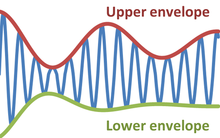
\includegraphics{./envelope.png}
 % envelope.png: 220x138 pixel, 96dpi, 5.82x3.65 cm, bb=0 0 165 104
  \label{envelopeFig}
\caption{Envelope superiore e inferiore di una onda sinusoidale\cite{envelopeImg}}
\end{figure}


\section{Funzione finestra}

Nell'elaborazione numerica dei segnali una funzione finestra \`e una funzione che vale zero al di fuori di un certo intervallo. Quando un'altra funzione \`e moltiplicata per una funzione finestra, anche il prodotto assume valori nulli al di fuori dell'intervallo. Una definizione pi\`u generale di funzione finestra non richiede l'annullarsi al di fuori di un intervallo, ma che il prodotto per la funzione di finestra sia una funzione a quadrato sommabile, ovvero che la funzione finestra si annulli in maniera sufficientemente rapida. Le funzioni finestra sono importanti nel progetto dei filtri FIR e nell'analisi spettrale. 

% \paragraph{analisi spettrale}
% La trasformata di Fourier della fuzione $cos(\omega t)$ \`e zero tranne che alle frequenze $\pm \omega$. Quindi molte funzioni e forme d'onda non hanno una forma chiusa conveniente dalla trasformata. Alternativamente si potrebbe essere interessati nel contenuto spettrale durante un certo intervallo di tempo. In entrambi i casi, la trasformata di Fourier pu\`o essere applicata su uno o pi\`u intervalli finiti nella forma d'onda. In generale la trasformata \`e applicata al prodotto della forma d'onda e alla finestra. Ogni finestra influisce sulla stima spettrale calcolata con questo metodo. 
% 
% \paragraph{windowing}
% L'applicazione di una finestra ad una forma d'onda semplice come ad esempio $cos(\omega t)$ fa si che la sua trasformata di Fourier abbia valori diversi da zero in frequenze di verse da $\omega$. 
% If the waveform under analysis comprises two sinusoids of different frequencies, leakage can interfere with the ability to distinguish them spectrally. If their frequencies are dissimilar and one component is weaker, then leakage from the larger component can obscure the weaker one’s presence. But if the frequencies are similar, leakage can render them unresolvable even when the sinusoids are of equal strength.

% The rectangular window has excellent resolution characteristics for sinusoids of comparable strength, but it is a poor choice for sinusoids of disparate amplitudes. This characteristic is sometimes described as low-dynamic-range.
% 
% At the other extreme of dynamic range are the windows with the poorest resolution. These high-dynamic-range low-resolution windows are also poorest in terms of sensitivity; this is, if the input waveform contains random noise close to the frequency of a sinusoid, the response to noise, compared to the sinusoid, will be higher than with a higher-resolution window. In other words, the ability to find weak sinusoids amidst the noise is diminished by a high-dynamic-range window. High-dynamic-range windows are probably most often justified in wideband applications, where the spectrum being analyzed is expected to contain many different components of various amplitudes.
% 
% In between the extremes are moderate windows, such as Hamming and Hann. They are commonly used in narrowband applications, such as the spectrum of a telephone channel. In summary, spectral analysis involves a tradeoff between resolving comparable strength components with similar frequencies and resolving disparate strength components with dissimilar frequencies. That tradeoff occurs when the window function is chosen.Discrete-time signals
% 
% When the input waveform is time-sampled, instead of continuous, the analysis is usually done by applying a window function and then a discrete Fourier transform (DFT). But the DFT provides only a coarse sampling of the actual DTFT spectrum. Figure 1 shows a portion of the DTFT for a rectangularly windowed sinusoid. The actual frequency of the sinusoid is indicated as "0" on the horizontal axis. Everything else is leakage, exaggerated by the use of a logarithmic presentation. The unit of frequency is "DFT bins"; that is, the integer values on the frequency axis correspond to the frequencies sampled by the DFT. So the figure depicts a case where the actual frequency of the sinusoid happens to coincide with a DFT sample,[note 1] and the maximum value of the spectrum is accurately measured by that sample. When it misses the maximum value by some amount (up to 1/2 bin), the measurement error is referred to as scalloping loss (inspired by the shape of the peak). But the most interesting thing about this case is 
% that all the other samples coincide with nulls in the true spectrum. (The nulls are actually zero-crossings, which cannot be shown on a logarithmic scale such as this.) So in this case, the DFT creates the illusion of no leakage. Despite the unlikely conditions of this example, it is a common misconception that visible leakage is some sort of artifact of the DFT. But since any window function causes leakage, its apparent absence (in this contrived example) is actually the DFT artifact.
% 
% [edit]Noise bandwidth
% The concepts of resolution and dynamic range tend to be somewhat subjective, depending on what the user is actually trying to do. But they also tend to be highly correlated with the total leakage, which is quantifiable. It is usually expressed as an equivalent bandwidth, B. Think of it as redistributing the DTFT into a rectangular shape with height equal to the spectral maximum and width B.[note 2][4] The more leakage, the greater the bandwidth. It is sometimes called noise equivalent bandwidth or equivalent noise bandwidth, because it is proportional to the average power that will be registered by each DFT bin when the input signal contains a random noise component (or is just random noise). A graph of the power spectrum, averaged over time, typically reveals a flat noise floor, caused by this effect. The height of the noise floor is proportional to B. So two different window functions can produce different noise floors.
% 
% [edit]Processing gain
% In signal processing, operations are chosen to improve some aspect of quality of a signal by exploiting the differences between the signal and the corrupting influences. When the signal is a sinusoid corrupted by additive random noise, spectral analysis distributes the signal and noise components differently, often making it easier to detect the signal's presence or measure certain characteristics, such as amplitude and frequency. Effectively, the signal to noise ratio (SNR) is improved by distributing the noise uniformly, while concentrating most of the sinusoid's energy around one frequency. Processing gain is a term often used to describe an SNR improvement. The processing gain of spectral analysis depends on the window function, both its noise bandwidth (B) and its potential scalloping loss. These effects partially offset, because windows with the least scalloping naturally have the most leakage.



% Le finestre vengono usate spesso nel progetto dei filtri digitali, in particolare per convertire 
% Windows are sometimes used in the design of digital filters, in particular to convert an "ideal" impulse response of infinite duration, such as a sinc function, to a finite impulse response (FIR) filter design. That is called the window method.[5][6]


% \subsection{Esempi di finestre}

% \paragraph{terminologia}
% Usiamo $N$ per rappresentare l'ampiezza in numero di campioni di una finestra simmetrica $w(n)$. Se $N$ \`e un numero dispari, la finestra non-flat ha un unico punto singolare massimo. Se $N$ \`e pari, ha un doppio massimo. 
% La finestra cosidetta DFT-pari \`e asimmetrica e ha un solo massimo ma un numero pari di campioni(richiesti dall'algoritmo FFT). 
% Each figure label includes the corresponding noise equivalent bandwidth metric (B)[note 2], in units of DFT bins. As a guideline, windows are divided into two groups on the basis of B. One group comprises 1 ≤ B ≤ 1.8, and the other group comprises B ≥ 1.98. The Gauss, Kaiser, and Poisson windows are parametric families that span both groups, though only one or two examples of each are shown.
% Ci sono varie finestre ad esempio: finestra rettangolare \`e la pi\`u semplice, lascia invariati i campioni al suo interno e mette a zero gli altri. 
$N$ rappresenta l'ampiezza, in numero di campioni, di una finestra a tempo discreto. Tipicamente \`e una potenza di 2. $n$ \`e un numero intero, che assume valori da $0$ ad $N-1$. Ci sono varie finestre ad esempio: 
\begin{itemize}
  \item 
    la finestra rettangolare descritta dall'equazione 
    \[
      w(n)=1  
    \]
  \item
    la finestra di Hamming descritta dall'equazione
    \[
    w(n)=0.54-0.46 cos \left(\frac{2 \pi n}{N-1}\right)
    \]
  \item
    la finestra di Hann o Hanning descritta dall'equazione:
    \[
      w(n)=0.5 cos \left(1-\frac{2 \pi n}{N-1}\right)
    \]
  \item
    la finestra di Blackmann descritta dall'equazione:
    \[
      w(n)=\frac{1-0.16}{2} - \frac{1}{2} cos \left(1-\frac{2 \pi n}{N-1}\right) + \frac{0.16}{2} cos \left(\frac{4 \pi n}{N-1}\right)
    \]
\end{itemize}

% Other windows are designed to moderate these sudden changes because discontinuities have undesirable effects on the discrete-time Fourier transform (DTFT) and/or the algorithms that produce samples of the DTFT.[9][10]

% \paragraph{finestra di Hamming}
\fi